%% Copyright 2015 by Clas Veibäck, Automatic Control, Linköping University

%% Notes on usage
%% With latex and sansserif fonts, pdfLaTeX can be used
%% With standard font, LuaLaTeX needs to be used and Calibri and Georgia need to be installed
%% With LiU font, LuaLaTeX needs to be used and Korolev LiU and Georgi need to be installed
%% With calibri font, LuaLaTeX needs to be used and Calibri need to be installed

%\documentclass[noamsthm, english]{beamer}
\documentclass[noamsthm, english]{beamer}

\usepackage[T1]{fontenc}
\usepackage{babel}
%\usepackage{pgfpages}

\usetheme[
%% Standard colors {blue, green, turquoise} for title, outline and end pages
titlecolor=blue,%
outlinecolor=green,%
endcolor=turquoise,%
%% Complementary colors {orange, purple, yellow, gray} for some details
complementary=orange,%
%% All colors {blue, green, turquoise, orange, purple, yellow, gray} for blocks
blockcolor=blue,%
%% Font schemes {latex, standard, sansserif, calibri, liu} to use
font=liu,%
%% Select color themes {highcontrast, superhighcontrast, dark} with high contrast or add handout option in documentclass
%highcontrast,%
%superhighcontrast,%
%% Remove outline before each section and end page with {nooutline, noendpage}
nooutline, %
%noendpage,%
%% Add navigation symbols with {navigation}
%navigation,%
%% Add total number of frames to frame count with {totalframes}
%totalframes,%
% Remove parts of header with {noheadertitle, noheaderauthor, noheaderdate, noheadernumber, minimalheader, noheader}
%noheadertitle,%
%noheaderauthor,%
%noheaderdate,%
%noheadernumber,%
%% Show institute in title frame
%showinstitute,
%% Show outline in two columns
%outlinecolumns,
]{LiU}

%% Add a text on end page, leave blank to add author
\finaltext{Thank you for YOUR time!}

%% Presentation information
\title[]{Exploring web protocols for use
on cellular networks}
\subtitle{QUIC on really poor network links}
\author{Hans-Filip Elo}
\institute{IDA \\
Your department \\
Linköping University}
\date{\today}

% Show notes on second screen
%\setbeameroption{show notes on second screen}
\setbeamertemplate{navigation symbols}{}

\begin{document}

\maketitle
\makeoutline

%\section{Section title}
%\subsection{Sub section title}

\section{Why does QUIC exist?}
\section{My test and my contributions}
\section{Results}


\begin{frame}

    \frametitle{Why does QUIC exist?}

    \note{Well, QUIC started with HTTP/2.}

    \begin{overprint}
        \uncover<+->{}
        \uncover<+->{
        HTTP/2 was created in order to shorten web latencies. HTTP/2 removes the limitation of HTTP/1.1 which only can send one resource at the time over a TCP connection. }
        ~\\
        ~\\
        \uncover<+->{
        Sending multiple resources over the same TCP connection is both what makes HTTP/2 perform better AND worse than HTTP/1.1.}
    \end{overprint}

\end{frame}

% -------------------------------------------

\begin{frame}
    \frametitle{Why does QUIC exist?}
    \begin{overprint}
        \framesubtitle{What? This makes no sense?}

        \uncover<+->{}
        \uncover<+->{
        On stable connections HTTP/2 performs objectively better when fetching many resources. In \href{https://http2.akamai.com/demo}{some edge cases} a lot better.}
        ~\\
        ~\\
        \uncover<+->{
        In most web browsing however the user can't notice the difference because of processing delay from their browser.}

        \note{According to Bocchi et al. This is a combination of actual processing delay limitations and that many web pages are optimized to work well with HTTP/1.1}


    \end{overprint}

\end{frame}

% -------------------------------------------
\begin{frame}
    \frametitle{Why does QUIC exist?}
    \framesubtitle{What about not so stable connections then?}

        \only<2>{
        Sending multiple resources over one TCP connection becomes a problem. A packet-loss or out-of-order packet for one resource stream causes head-of-line blocking.}

\end{frame}

% ----------------------------------

\begin{frame}
    \frametitle{Why does QUIC exist?}
    \framesubtitle{What about not so stable connections then?}
    \begin{overprint}

        \uncover<+->{}
        \only<2>{
        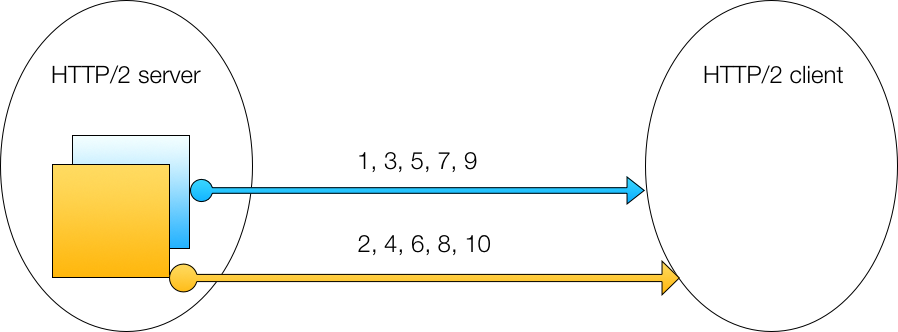
\includegraphics[width=0.9\textwidth]{figures/http2-two-resources.png}}
        \only<3,4>{
        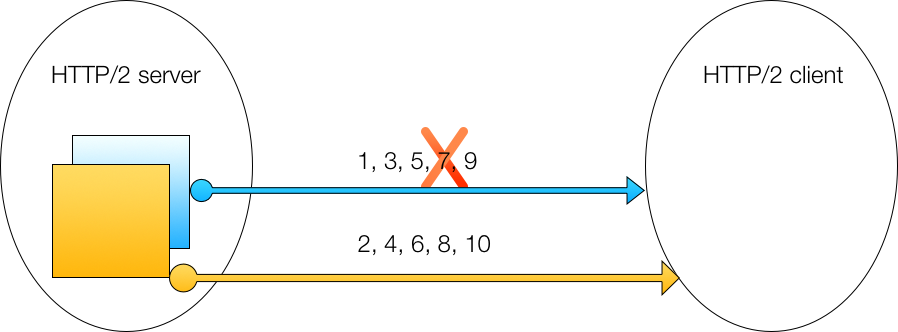
\includegraphics[width=0.9\textwidth]{figures/http2-two-resources-packet-loss.png}}
        \only<4>{
        Head-of-line blocking is introduced since the TCP connection counts every packet with a index higher than the lost packet as ``not arrived yet''.}

    \end{overprint}

\end{frame}


% ----------------------------------
\begin{frame}
    \frametitle{Why does QUIC exist?}
    \framesubtitle{QUIC improvements over HTTP/2}

    \begin{overprint}
        \uncover<+->{}

        \begin{itemize}
            \uncover<+->{
            \item QUIC includes per-stream congestion control, avoiding head-of-line blocking.}
            \uncover<+->{
            \item QUIC has way faster connection setup times (0-1 RTT vs 3 RTT).}
            \uncover<+->{
            \item Connection migration. Allows connection to continue even if user changes IP-address (moving between LTE/WiFi for example).}
            \uncover<+->{
            \item Forward error correction.}
        \end{itemize}

    \end{overprint}

\end{frame}



\begin{frame}
    \frametitle{My testbed}
    \framesubtitle{QUIC sounds great, but is it?}

    \begin{overprint}
        \uncover<+->{}

        \uncover<+->{
    I've been testing QUIC in limited network scenarios in order to explore how QUIC performs during web browsing over poor network conditions.}
        ~\\
        ~\\
        \uncover<+->{Available measurements of QUIC seems to focus mostly on the best-case scenarios for QUIC and HTTP/2 with high bandwidth-delay product. }
    \end{overprint}

\end{frame}

% ------------------------------------

\begin{frame}
    \frametitle{My testbed}
    %\framesubtitle{}

    \begin{overprint}
        \uncover<+->{}

        \uncover<+->{\center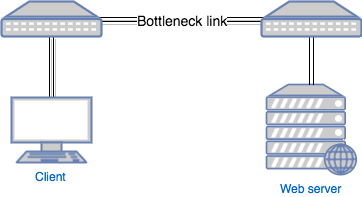
\includegraphics[width=0.7\textwidth]{../master-thesis/figures/testbench.pdf}}

    \end{overprint}

\end{frame}

% ------------------------------------

\begin{frame}
    \frametitle{My testbed}
    %\framesubtitle{}

    \begin{overprint}
        \uncover<+->{}

        \uncover<+->{Loads pre-downloaded content from 42 of Alexas top 100 webpages over a virtualized bottleneck link.}
        ~\\
        ~\\
        \uncover<+->{Measures network load times and how much data the browser managed to fetch.}
        ~\\
        ~\\
        \uncover<+->{Uses 16 different scenarios, each tested with both a persistent connection as well as a new connection for each page load.} \note{Scenario here means different properties of the bottleneck link.}

    \end{overprint}

\end{frame}

% ------------------------------------

\begin{frame}
    \frametitle{My testbed}
    \framesubtitle{Scenario categories}

    \begin{overprint}
        \uncover<+->{}
        \begin{itemize}
                \uncover<+->{
                \item Baseline}
                \uncover<+->{
                \item Bandiwdth limited}
                \uncover<+->{
                \item Latency added}
                \uncover<+->{
                \item Loss added}
        \end{itemize}
    \end{overprint}

\end{frame}


\end{document}
